\documentclass[10pt]{article}
\usepackage{graphicx}
\usepackage[T1]{fontenc}
\usepackage[utf8]{inputenc}
\usepackage[letterpaper,margin=1in]{geometry}
\usepackage[parfill]{parskip}

\begin{document}

\title{\textbf{\Large{\textsc{ECE320:} Fields and Waves}} \\ \Large{Lab 1 Report: Waves on Transmission Lines}}
\author{Alp Tarım, Pranshu Malik}


\maketitle

\section{Introduction}
This assignment was about exploring the characteristics of transmission lines (abbrv. T.L.), studying voltage and current 
propagation along the T.L.s, as well as depedance on loads.

Introduction to the lab and its purpose. The following is the reflection coefficient for a transmission line

\[
    \label{simple_equation}
    \Gamma = \frac{Z_L - Z_0}{Z_L + Z_0}
\]

\section{Determining the Characteristic Impedance, $Z_0$}

Lorem ipsum dolor sit amet, consectetur adipisicing elit, sed do eiusmod tempor
incididunt ut labore et dolore magna aliqua. Ut enim ad minim veniam, quis
nostrud exercitation ullamco laboris nisi ut aliquip ex ea commodo consequat.
Duis aute irure dolor in reprehenderit in voluptate velit esse cillum dolore eu
fugiat nulla pariatur.

We know that the reflections become 0 when $Z_L = Z_0$.

\begin{figure}
    \centering
    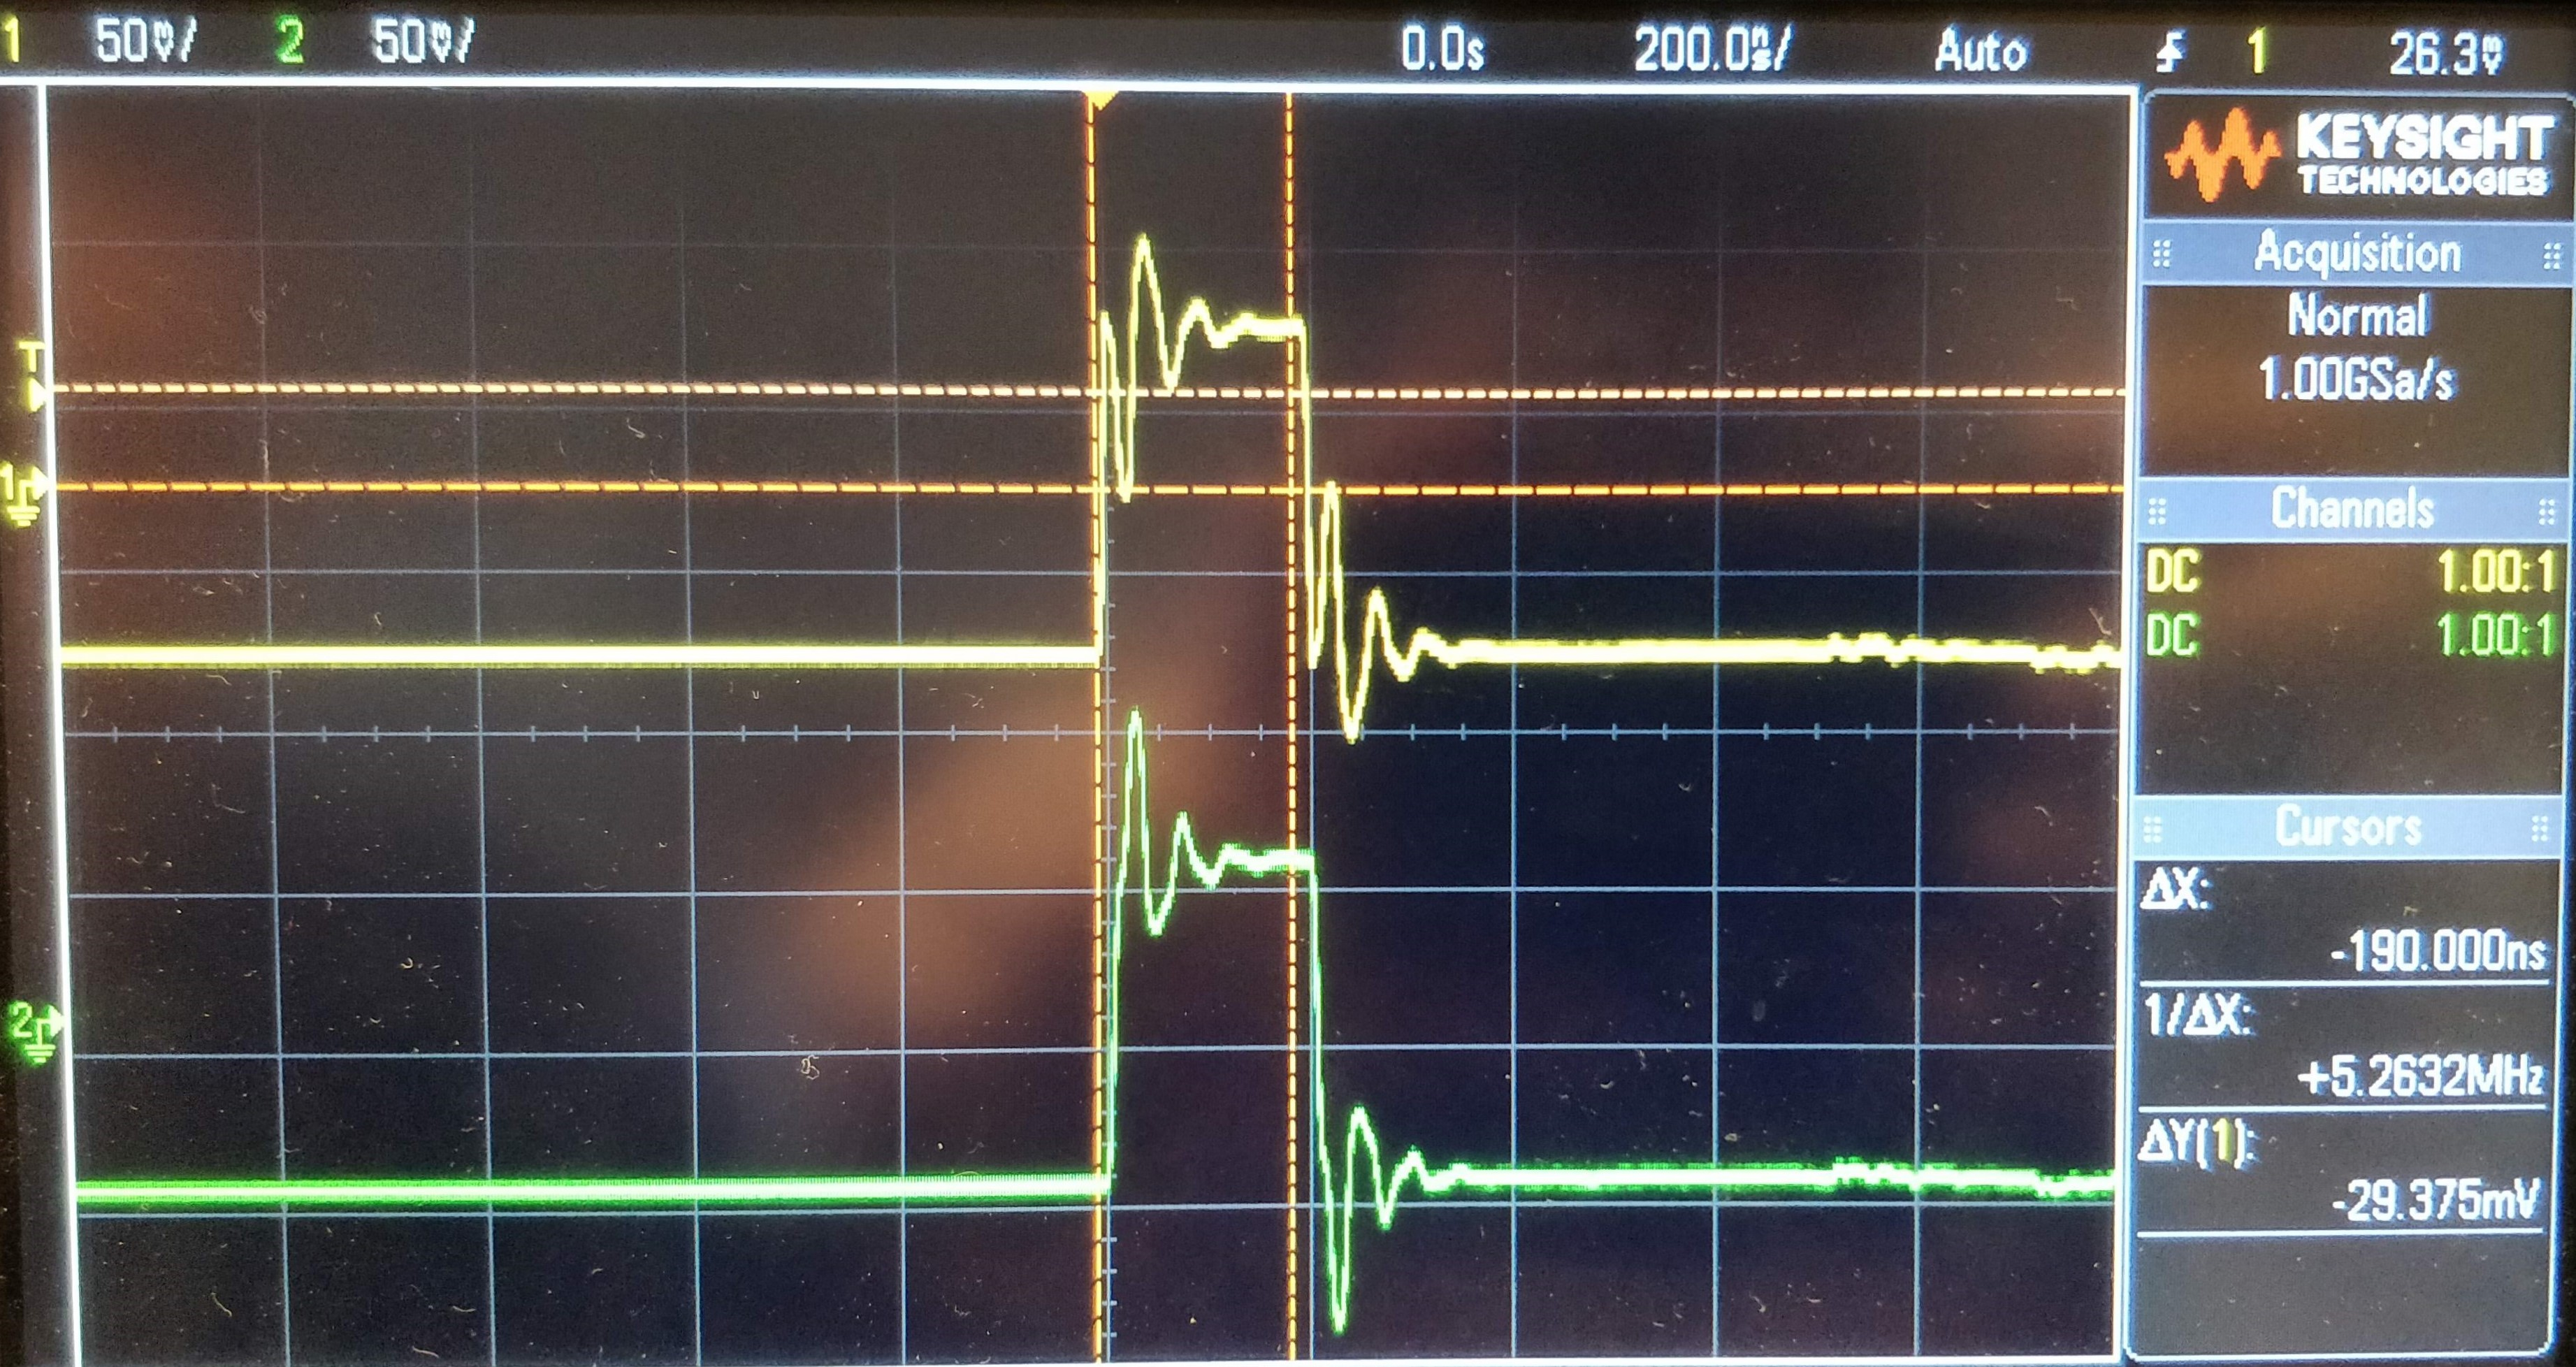
\includegraphics[width=3.0in]{photos/lab1/test.jpg}
    \caption{Simulation Results}
    \label{simulationfigure}
\end{figure}


\section{Conclusion}

Lorem ipsum dolor sit amet, consectetur adipisicing elit, sed do eiusmod tempor
incididunt ut labore et dolore magna aliqua. Ut enim ad minim veniam, quis
nostrud exercitation ullamco laboris nisi ut aliquip ex ea commodo consequat.
Duis aute irure dolor in reprehenderit in voluptate velit esse cillum dolore eu
fugiat nulla pariatur.


\end{document}